\section{Results}


\subsection{Experiment 1: General Benchmark}

Table \ref{tab:tuned-benchmark} and Figure \ref{fig:benchmark-perf} present the test accuracy of various methods in a 5-way, 5-shot setting for two datasets. In this setting, methods without the SOT module achieve an average accuracy of 87\% on the \texttt{TM} dataset and 66\% on the \texttt{SP} dataset, providing a strong baseline performance.

Moreover, the inclusion of the SOT module improves the performance of all methods, except for the Baseline. The \texttt{B++} method shows only a slight enhancement with SOT. In contrast, the other three methods benefit significantly from SOT, with an average performance increase of 12\% for \texttt{TM} and 48\% for \texttt{SP}. This indicates a considerable effect size from integrating the SOT module in both datasets.

\begin{table}[ht]
\caption{
    \textbf{Benchmark Results.} Test accuracy of all methods on \texttt{TM} and \texttt{SP} in the 5-way-5-shot setting. We depict the average accuracy and the 95\% confidence interval both without (left) and with SOT (right) and the difference.
    \vspace{5pt}
}

\label{tab:tuned-benchmark}
\centering
\begin{tabular}{llllr}
\toprule
 &  & \multicolumn{2}{@{}c}{\textbf{Test Acc. (\%)}} & \\
 &  & w/o SOT & w/ SOT & Diff \\
\midrule
\multirow[c]{5}{*}{\texttt{TM}} & B & $90.7 \pm 0.7$ & $86.3 \pm 0.9$ & {\color{red} +4.8} \\
 & B++ & $81.9 \pm 0.9$ & $82.8 \pm 0.9$ &  {\color{teal} +1.1} \\
 & MAML & $\mathbf{92.8} \pm 0.5$ & $99.2 \pm 0.1$ & {\color{teal} +6.9} \\
 & MN & $84.6 \pm 0.8$ & $\mathbf{99.7} \pm 0.1$ &  {\color{teal} +17.9} \\
 & PN & $87.1 \pm 0.8$ & $98.6 \pm 0.2$ & {\color{teal} +13.2} \\
\midrule
\multirow[c]{5}{*}{\texttt{SP}} & B & $\mathbf{69.2} \pm 0.7$ & $55.7 \pm 0.8$ & {\color{red} -19.6} \\
 & B++ & $64.1 \pm 0.7$ & $64.6 \pm 0.7$ & {\color{teal} +0.8} \\
 & MAML & $68.7 \pm 0.7$ & $98.0 \pm 0.2$ & {\color{teal} +42.8} \\
 & MN & $68.2 \pm 0.8$ & $\mathbf{99.8} \pm 0.1$ & {\color{teal} +46.5} \\
 & PN & $63.5 \pm 0.7$ & $99.2 \pm 0.1$ & {\color{teal} +56.1} \\
\bottomrule
\end{tabular}
\end{table}

\subsection{Experiment 2: Way-Shot Analysis}

Figure \ref{fig:way-shot} illustrates the results of the way-shot analysis, displaying test accuracy in relation to the number of classes (left subplot) and the number of samples (right subplot).

Predictably, in the absence of the \texttt{SOT} module, accuracy diminishes as the number of ways increases and rises with more shots. Conversely, with the \texttt{SOT} module, accuracy remains consistent across varying numbers of ways and shots.

\begin{figure}[h!]
    \centering
    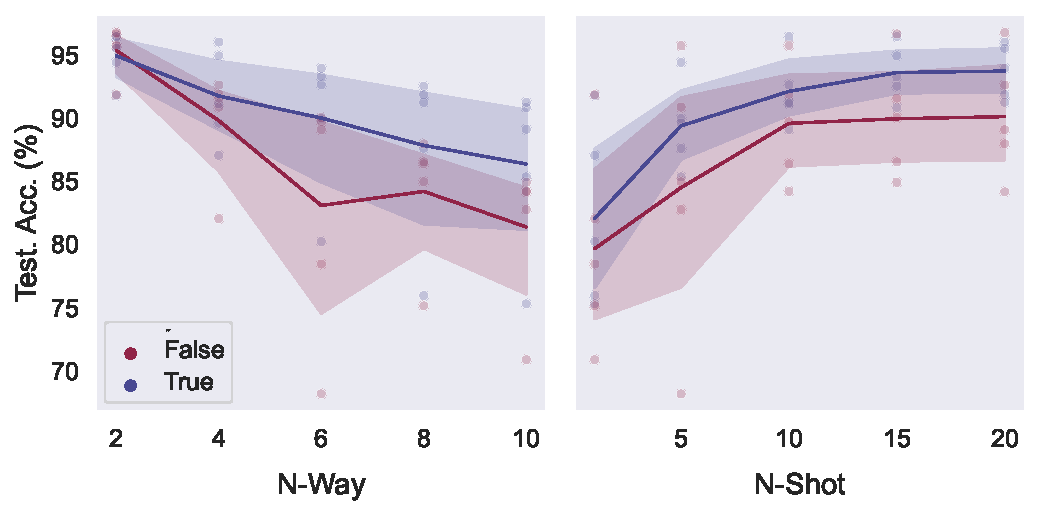
\includegraphics[width=1\columnwidth]{../figures/way-shot.pdf}
    \caption{Test accuracy of the \texttt{ProtoNet} method on the \texttt{TM} dataset with and without the \texttt{SOT} module in various few-shot learning settings for fixed n-way (left) and n-shot (right). Individual points represent a single experiment, the line is the regression line and the shaded area is the 95\% confidence interval.}
    \label{fig:way-shot}
\end{figure}

\subsection{Experiment 3: SOT integration}

In Figure \ref{fig:sot-interaction-scatter}, we illustrate the performance of various 
configurations of the \texttt{MatchingNet} method with and without the \texttt{SOT} 
module. Firstly, it is evident that without any form of embedding, regardless of the presence or 
absence of the \texttt{SOT} module, the performance is only 40\%. Secondly, in the absence of the 
\texttt{SOT} module, the optimal performance is achieved through the embedding of support vectors. 
Slightly inferior performance is observed when the query vectors are embedded. 
Most notably, the \texttt{SOT} module enhances the performance of all configurations. 
However, the optimal performance is attained in configurations where at least one of the 
support or query vectors is embedded.

\begin{figure}[h!]
    \centering
    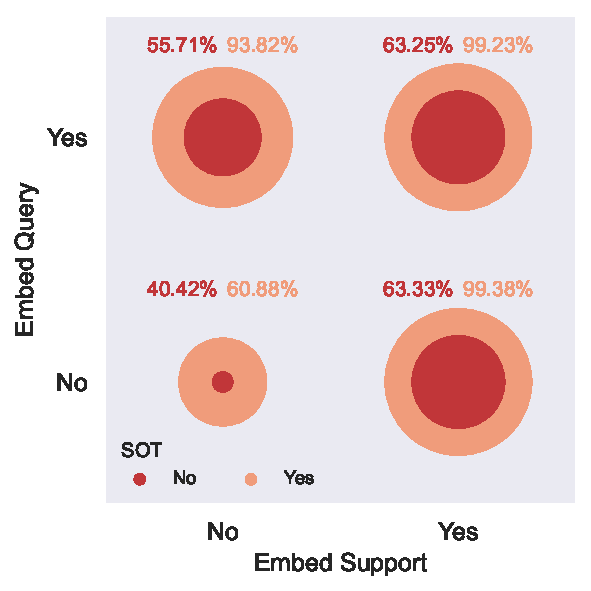
\includegraphics[width=0.75\columnwidth]{../figures/sot-interaction-scatter.pdf}
    \caption{Performane of different configurations of MatchingNet with and without SOT on the Tabula Muris dataset.}
    \label{fig:sot-interaction-scatter}
\end{figure}

\begin{figure*}
    \centering
    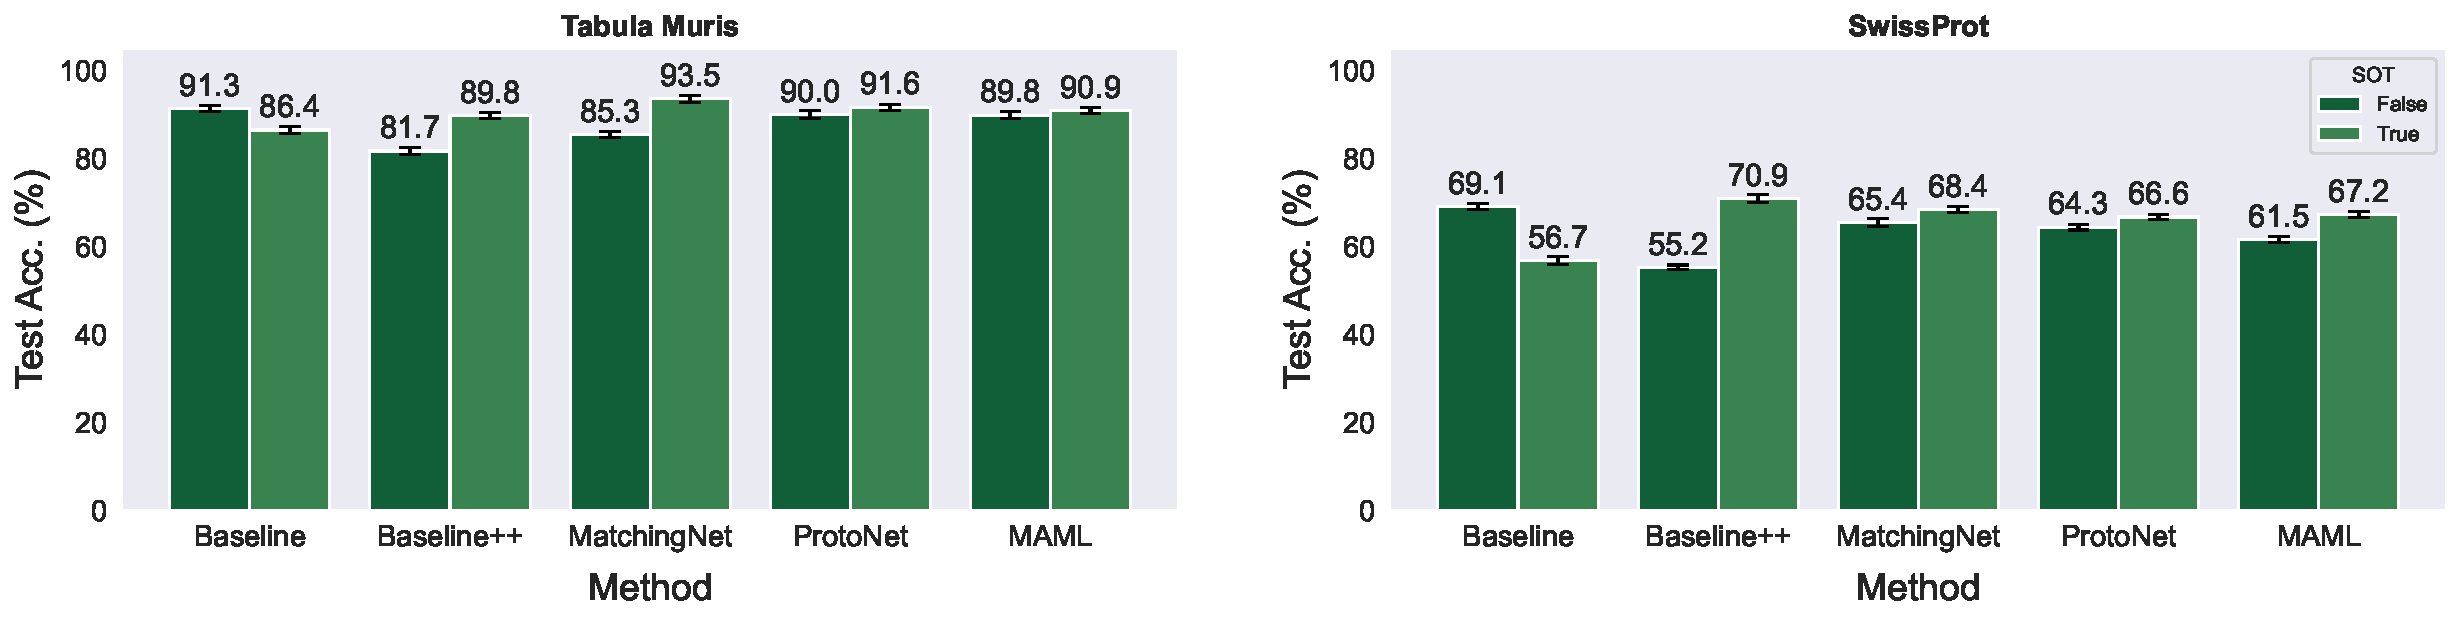
\includegraphics[width=0.9\linewidth]{../figures/benchmark-perf.pdf}
    \caption{Test accuracy of all methods on \texttt{TM} (left) and \texttt{SP} (right) in the 5-way-5-shot setting.}
    \label{fig:benchmark-perf}
\end{figure*}